\section{Resultados}
	
\subsection{Hardware}

	Como afirmado anteriormente, o primeiro passo do projeto é a prototipagem do Hardware do sistema, que inclui o Arduino, os botões e potenciômetros, através da plataforma online TinkerCAD, que inclui em si um monitor serial para visualizar o que está sendo enviado serialmente pelo microcontrolador.

\begin{figure}[htbp]
     \centerline{
        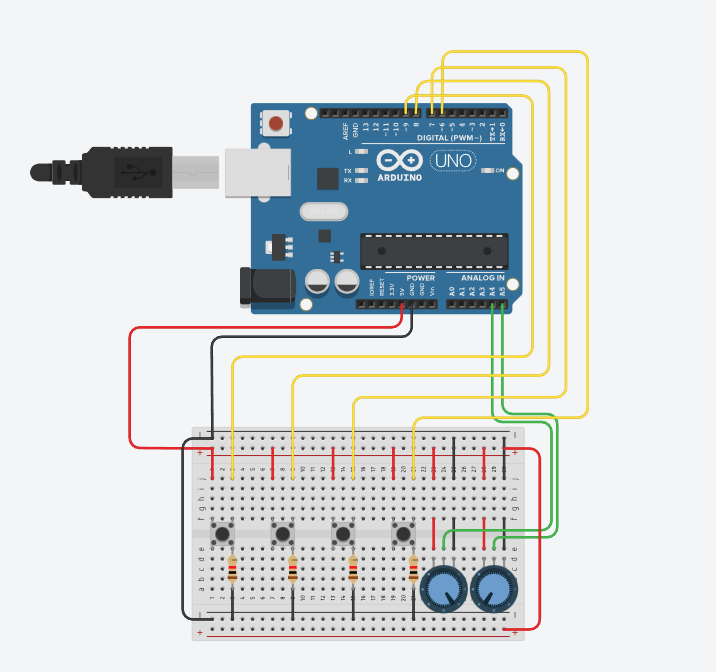
\includegraphics[width=2in]{tinkercad.png}
        }
     \caption{Modelo prototipado no TinkerCAD.}
     \label{fig}
    \end{figure}

	Como pode ser visto na figura acima, o modelo foi criado para abrigar dois potenciômetros e uma quantidade de botões, que foram 4 no momento da simulação. Cada um destes associados a um pino digital respectivo. Assim, a função do Arduino será pegar as informações desses componentes eletrônicos e enviar serialmente para o computador serialmente. O que tornará isso possível é a utilização da biblioteca "softwareserial.h" e suas funções, que possibilitam a comunicação.
	
	Para enviar todas as informações de uma única vez, em um pacote só, elas serão inseridas em uma string, e sua separação será realizada no código do Processing. Assim sendo, o código inserido no Arduino compreende a seguinte lógica:

\begin{lstlisting}[language=C]
const int pot1 = A5, pot2 = A3; //Potenciometros
const int b01 = 8, b02 = 7; // Botoes
int v_pot1 = 0, v_pot2 = 0; //Valores dos potenciometros
bool v_b01,v_b02; //Valores dos Botoes
int arr[10];

void setup() {
  Serial.begin(9600);
  pinMode(pot1, INPUT);
  pinMode(pot2, INPUT);
  for(int i = 7; i <= 8; i++){
      pinMode(i, INPUT_PULLUP);
    }
}

void loop() {
  v_pot1 = map(analogRead(pot1),0,1023,0,255);
  Serial.print(String(v_pot1) + "-");
  v_pot2 = map(analogRead(pot2),0,1023,0,255);
  Serial.print(String(v_pot2) + "-");
  v_b01 = !digitalRead(b01);
  v_b02 = !digitalRead(b02);
  Serial.print(String(v_b01) + "-");
  Serial.print(String(v_b02) + "\n");
  delay(50);
}
\end{lstlisting}

	Além da declaração de variáveis, alguns recursos foram utilizados para saber por exemplo, se um botão estava sendo pressionado. Como ele está pinado em uma porta digital, é possivel utilizar uma propriedade chamada "INPUT\_PULLUP"	para fazer essa distinção. Isso ocorre já que o botão está conectado a um resistor de "Pull-Up", que está inbutido no Arduino UNO, e quando vemos a expressão abaixo, significa que essa resistência irá impactar naquele input quando acionado, atuando como um inversor, para assim se obter um nível lógico alto quando o botão é pressionado:

\begin{lstlisting}[language=C]
pinMode(i, INPUT_PULLUP);
\end{lstlisting}

	Coletadas as informaçãos, elas são adicionadas a uma string de modelo: [x-x-x-x], e esta será separada por uma lógica criada na programação em Processing, transformando-as em chars, e associando-as às suas respectivas classes/variáveis.

	Por fim, para acomodar os potenciômetros e botões, foi impresso em 3D um modelo de controle "joystick" chamado "Paddle Game Controller" apropriado para o "Pong", visto abaixo:

\begin{figure}[htbp]
     \centerline{
        \includegraphics[width=2in]{botão.png}
        }
     \caption{Controle impresso 3D para o jogo.}
     \label{fig}
    \end{figure}

\begin{figure}[htbp]
     \centerline{
        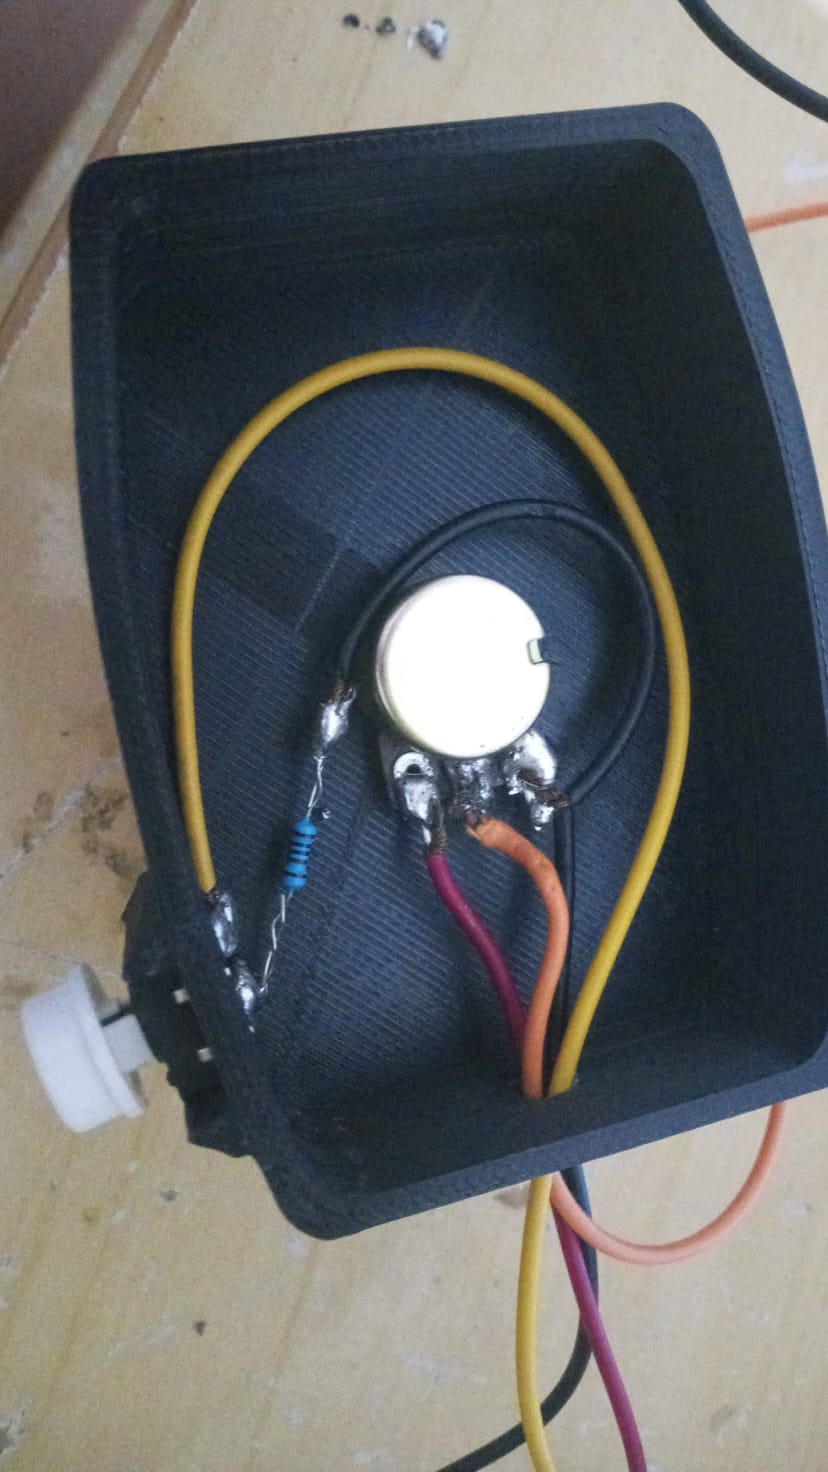
\includegraphics[width=2in]{solda.jpeg}
        }
     \caption{Eletrônicos soldados no controle.}
     \label{fig}
    \end{figure}

	

\subsection{Software/Processing}

	Antes de dar continuidade, é necessário estabelecer o que é desejado para o jogo: Uma tela inicial, que pode levar ao jogo em si ou a um menu de instruções, e que o jogo possa ser pausado.
	
	%%desenvolvimento

\begin{figure}[htbp]
     \centerline{
        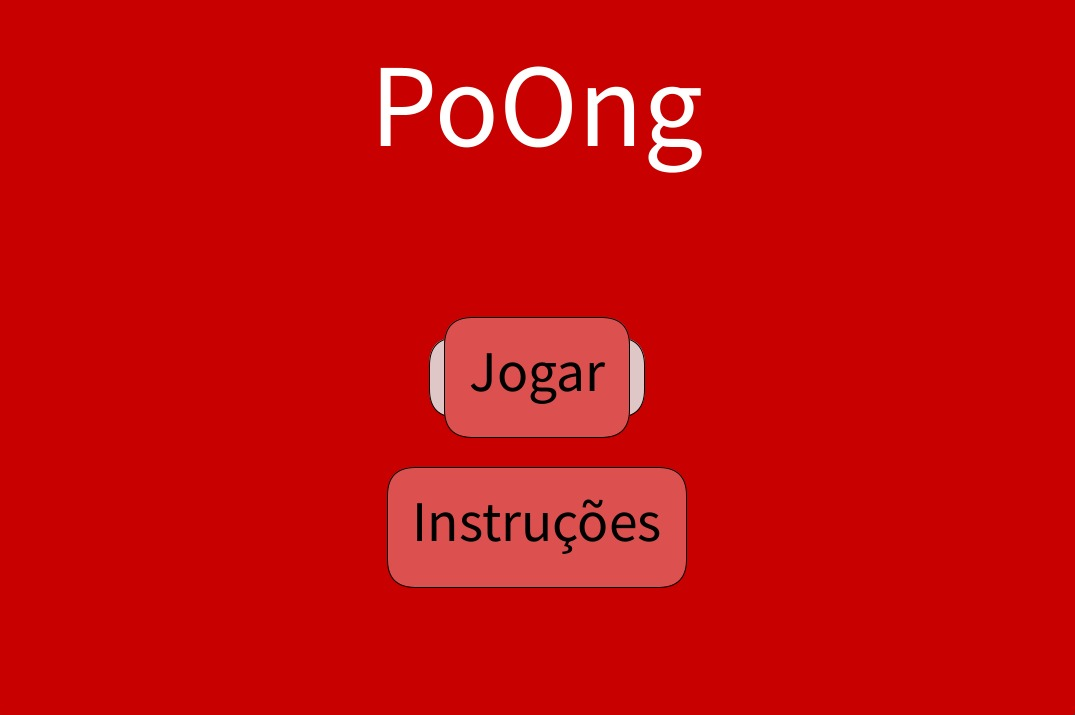
\includegraphics[width=3in]{tela-inicial.jpeg}
        }
     \caption{Tela inicial do jogo.}
     \label{fig}
    \end{figure}





